\documentclass[12pt,letterpaper]{article}
\usepackage[utf8]{inputenc}
\usepackage[spanish]{babel}
\usepackage{graphicx}
\usepackage{tabularx}
\usepackage{multirow}
\usepackage{float}
\usepackage{hyperref}
\usepackage{enumerate} 

\begin{document}
\begin{center}
{\Large \textbf{Métodos Computacionales - Taller 4}}\\
\vspace{0.3cm}
\textbf{Julián Leandro Rodríguez Cardona - 201416065}\\ \vspace{0.3cm}
29 de Abril del 2017
\end{center}

\section*{Ecuación de difusión de calor}

A continuación se presentan las gráficas obtenidas al resolver la ecuación de difusión de calor para una placa cuadrada de un metro, la cual inicialmente tiene un segmento rectangular con una temperatura mayor al resto de la placa. Esto se realizó para dos casos:

\begin{itemize}
\item El segmento rectangular a una temperatura de 100 $^{\circ}$C y el resto de la placa a una de 50 $^{\circ}$C. Estos valores solo eran iniciales, es decir, toda la placa está sujeta a posibles cambios.
\item El segmento rectangular a una temperatura de 100 $^{\circ}$C y el resto de la placa a una de 50 $^{\circ}$C. Sin embargo, se supone que existe una fuente de calor que permite que el segmento rectangular permanezca con la misma temperatura inicial.
\end{itemize}

Lo anterior se hizo para distintas condiciones de frontera:\\

\begin{itemize}
\item Fijas a 50 $^{\circ}$C.
\item Abiertas
\item Periódicas
\end{itemize}

Al realizar las simulaciones se pudo notar que con un coeficiente de difusión $\nu= 10^{-4}$, tal como se sugiere en el enunciado, los cambios son mínimos. Si se modifica este coeficiente por uno un poco mayor, los cambios de temperatura respecto al tiempo comienzan a evidenciarse mucho mejor. Por lo tanto, en los siguientes resultados se utiliza un $\nu=0.1$ con el cual se puede observar mejor los cambios que se producen.

\section*{Condiciones de frontera fijas}

\subsection*{Caso 1}

\begin{figure}[H]
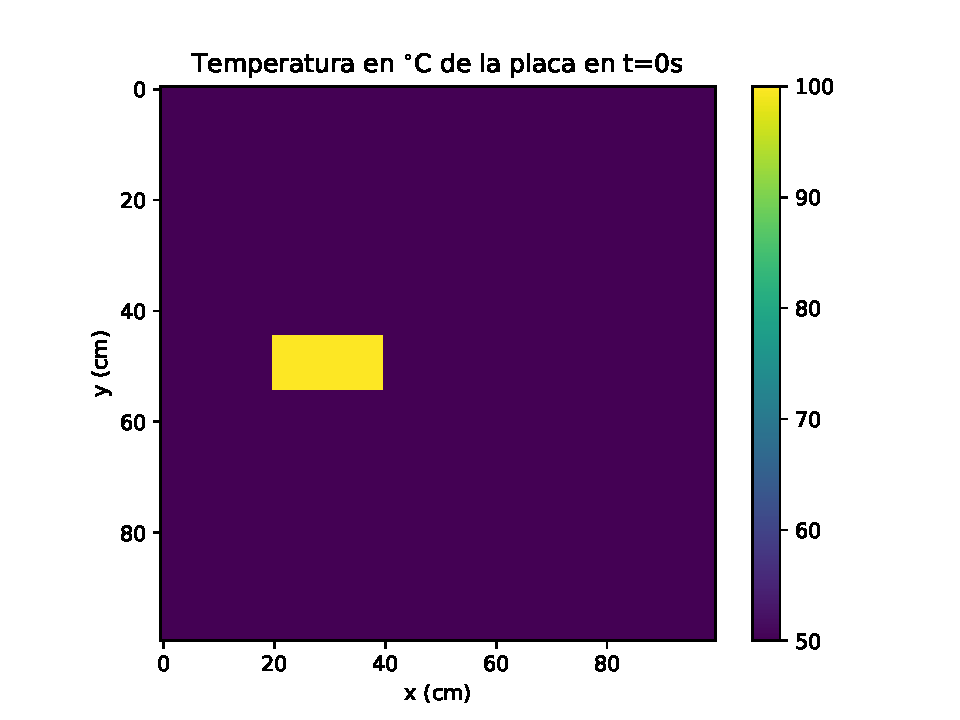
\includegraphics{f1_0.pdf}
\centering
\end{figure}

\begin{figure}[H]
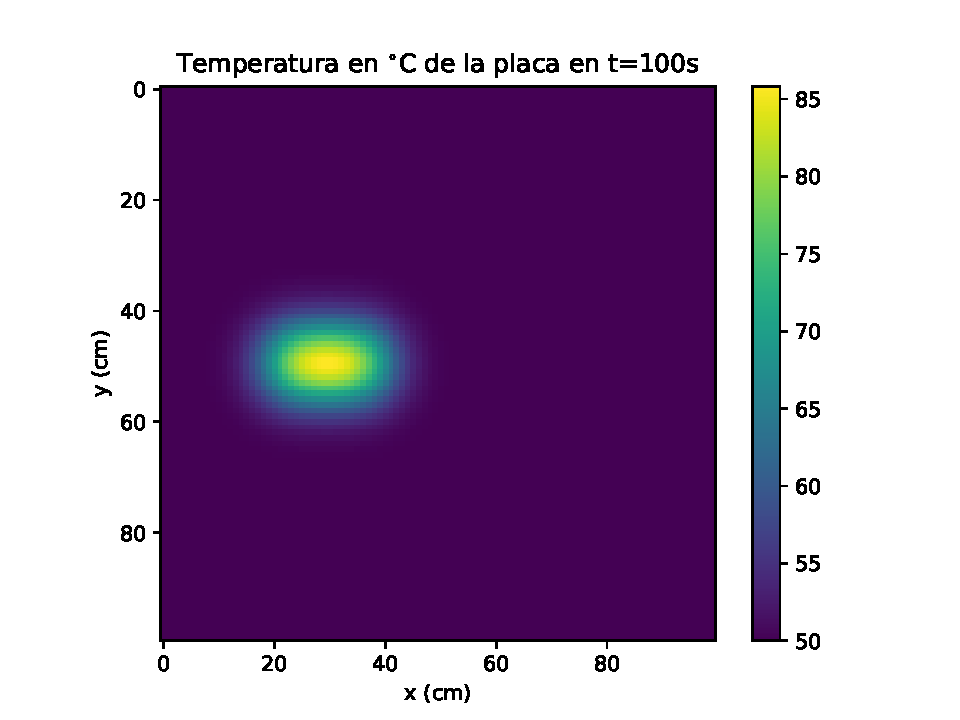
\includegraphics{f1_100.pdf}
\centering
\end{figure}

\begin{figure}[H]
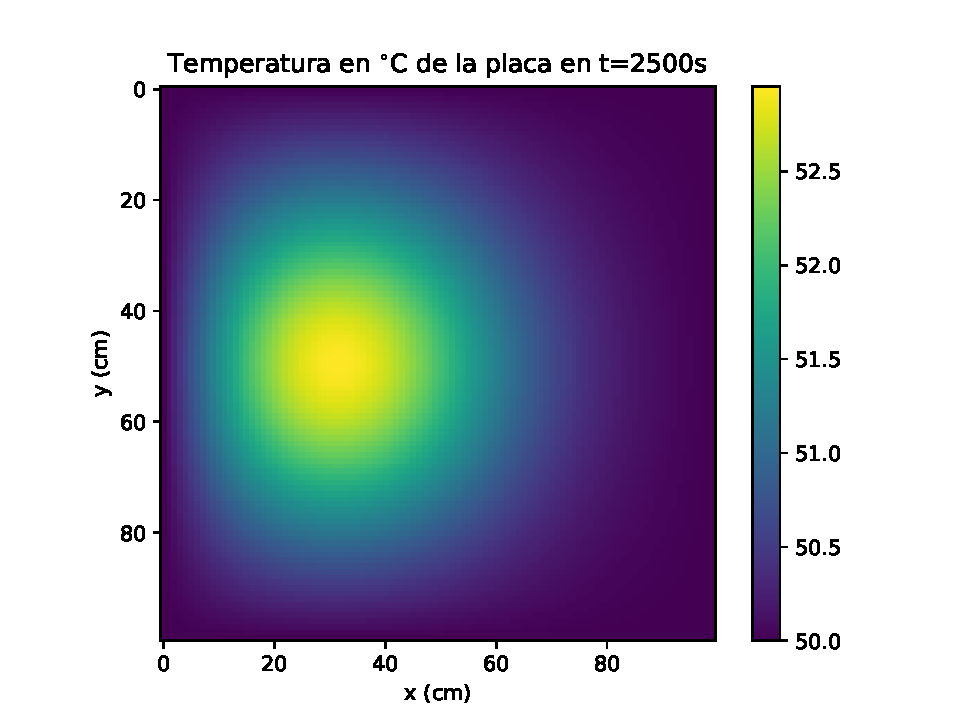
\includegraphics{f1_2500.pdf}
\centering
\end{figure}

\subsection*{Caso 2}

\begin{figure}[H]
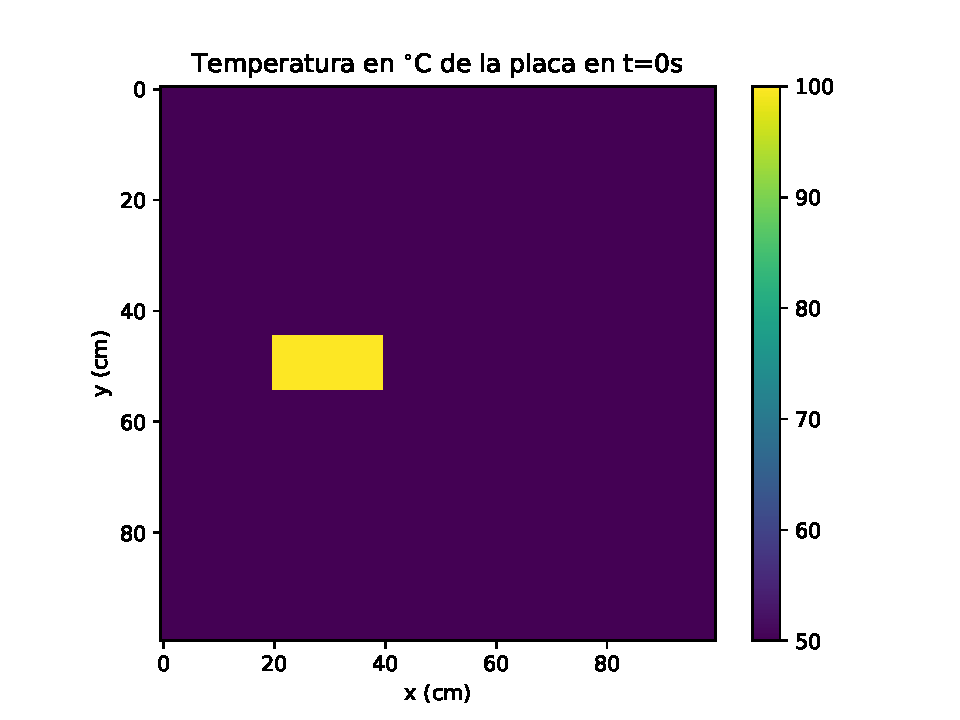
\includegraphics{f2_0.pdf}
\centering
\end{figure}

\begin{figure}[H]
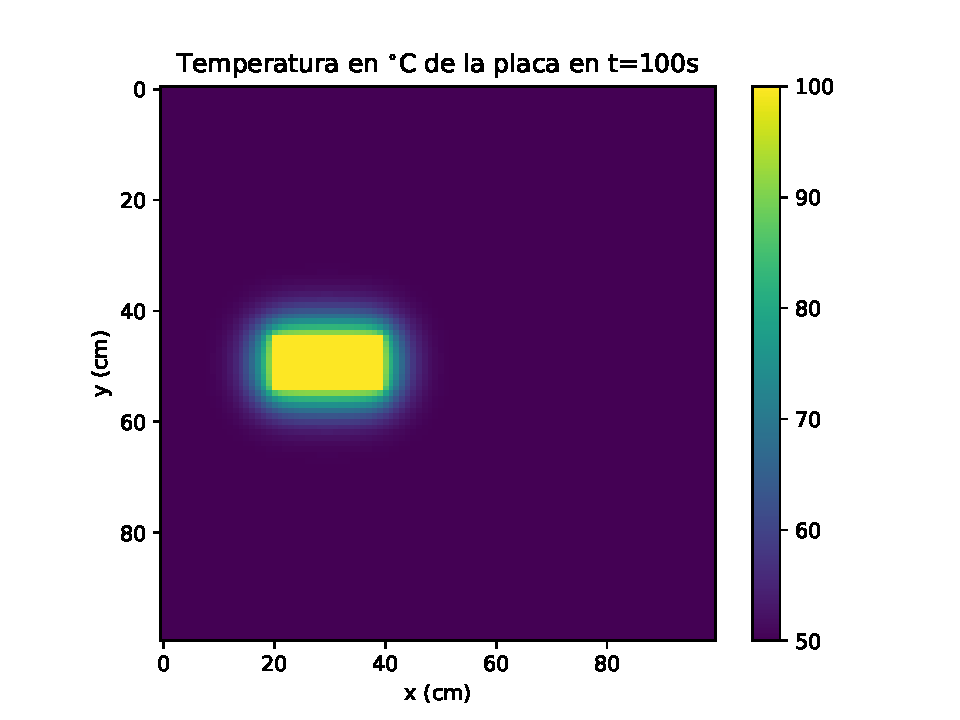
\includegraphics{f2_100.pdf}
\centering
\end{figure}

\begin{figure}[H]
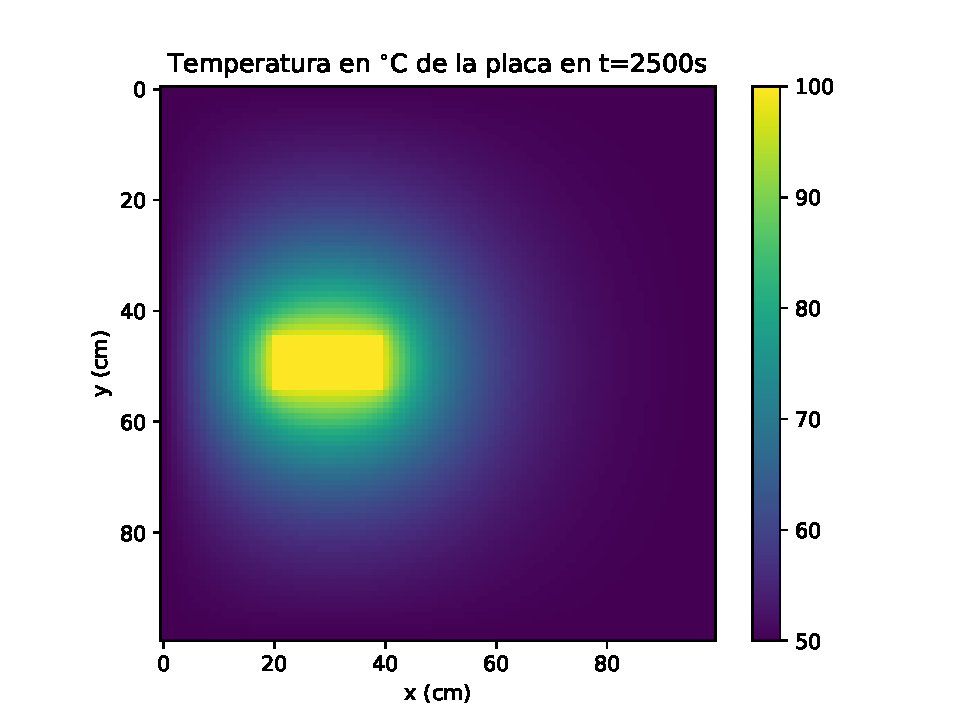
\includegraphics{f2_2500.pdf}
\centering
\end{figure}

\section*{Condiciones de frontera abiertas}

\subsection*{Caso 1}

\begin{figure}[H]
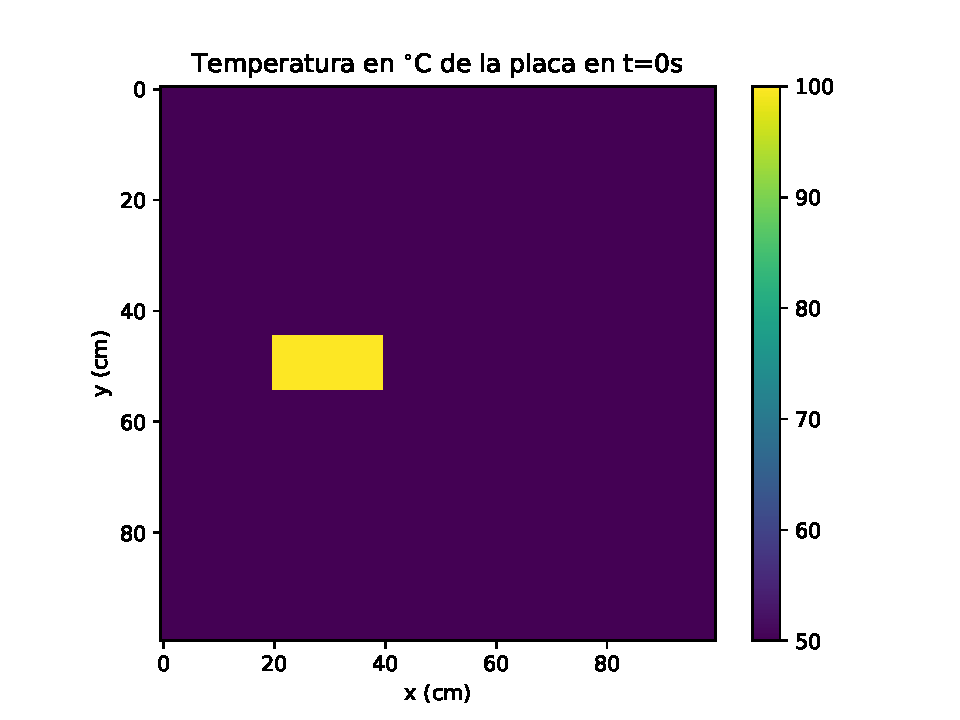
\includegraphics{a1_0.pdf}
\centering
\end{figure}

\begin{figure}[H]
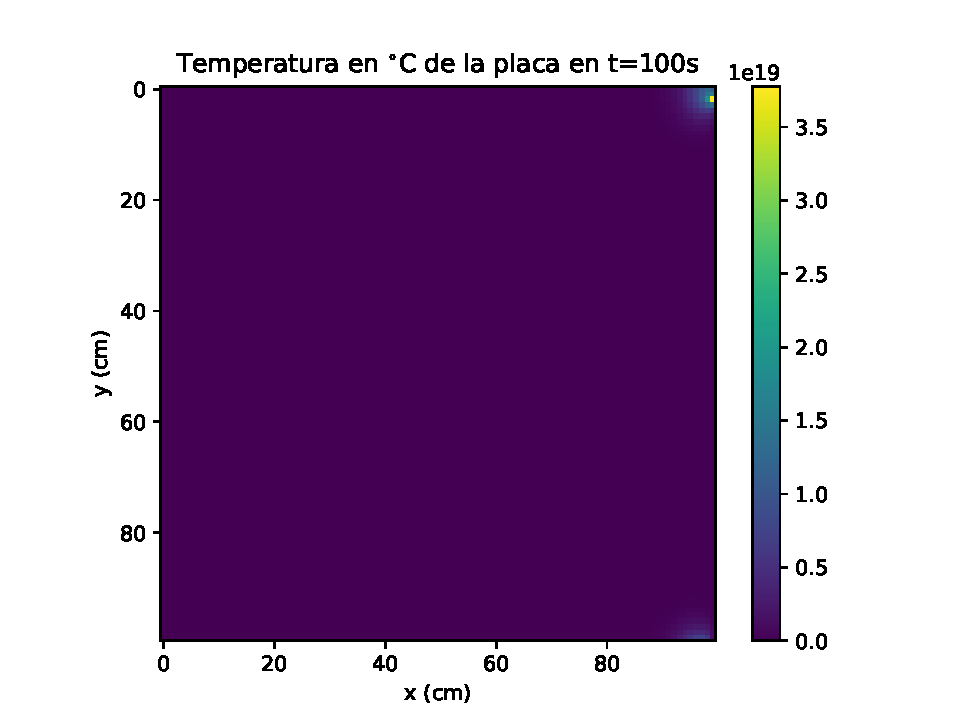
\includegraphics{a1_100.pdf}
\centering
\end{figure}

\begin{figure}[H]
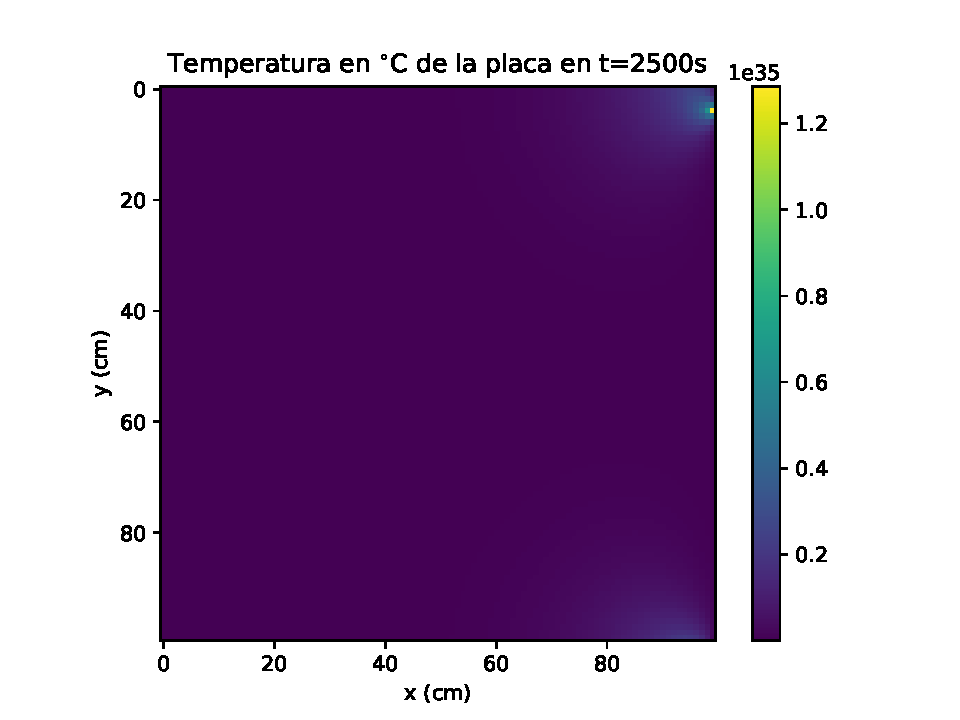
\includegraphics{a1_2500.pdf}
\centering
\end{figure}

\subsection*{Caso 2}

\begin{figure}[H]
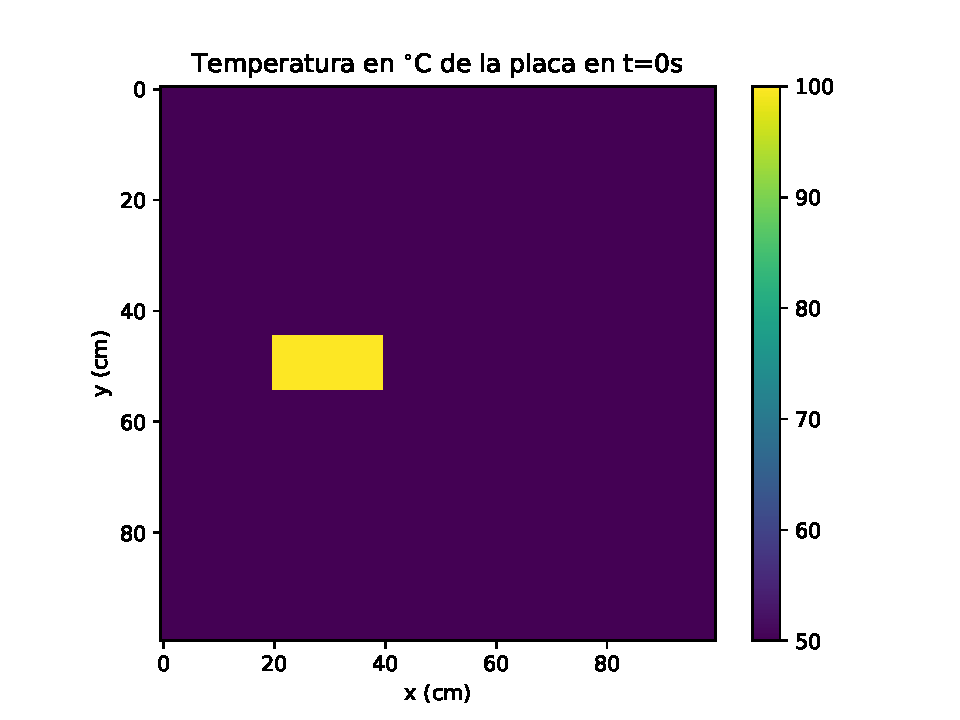
\includegraphics{a2_0.pdf}
\centering
\end{figure}

\begin{figure}[H]
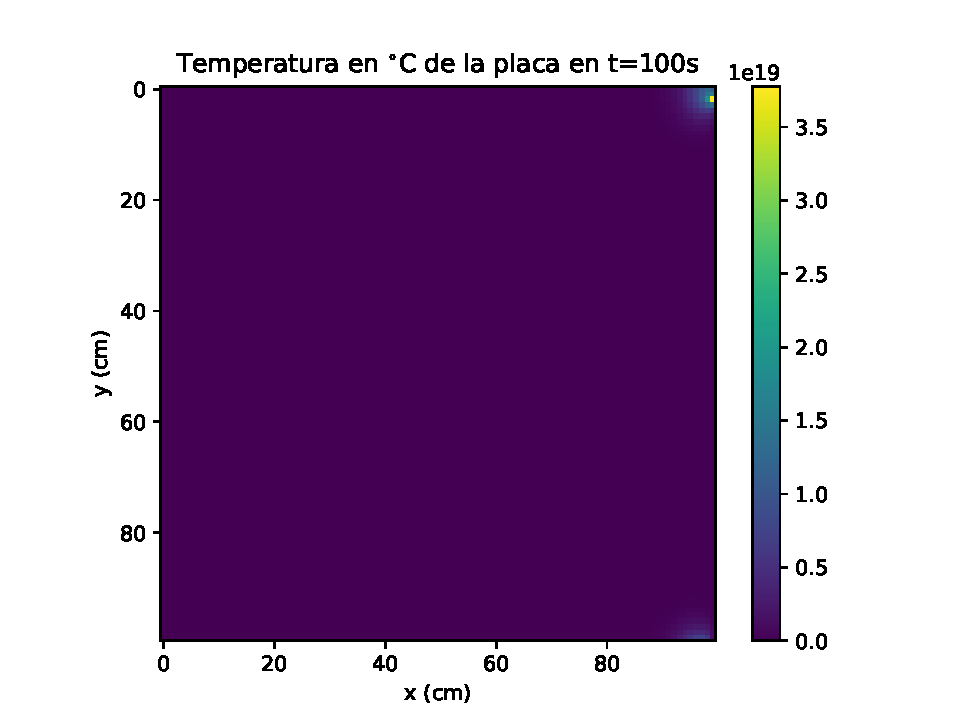
\includegraphics{a2_100.pdf}
\centering
\end{figure}

\begin{figure}[H]
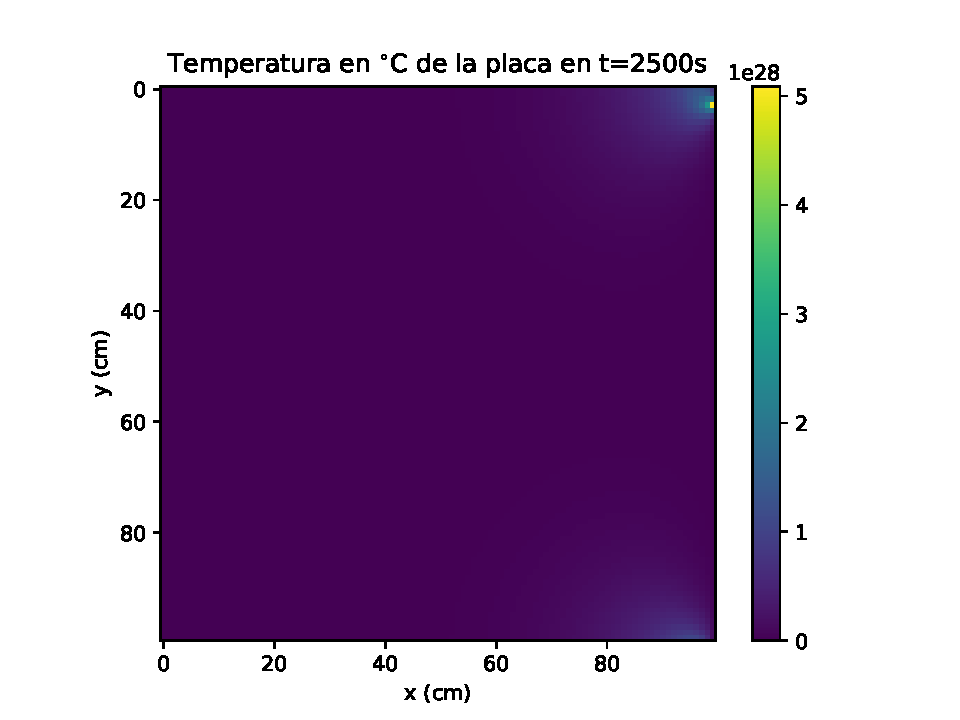
\includegraphics{a2_2500.pdf}
\centering
\end{figure}

\section*{Condiciones de frontera periódicas}

\subsection*{Caso 1}

\begin{figure}[H]
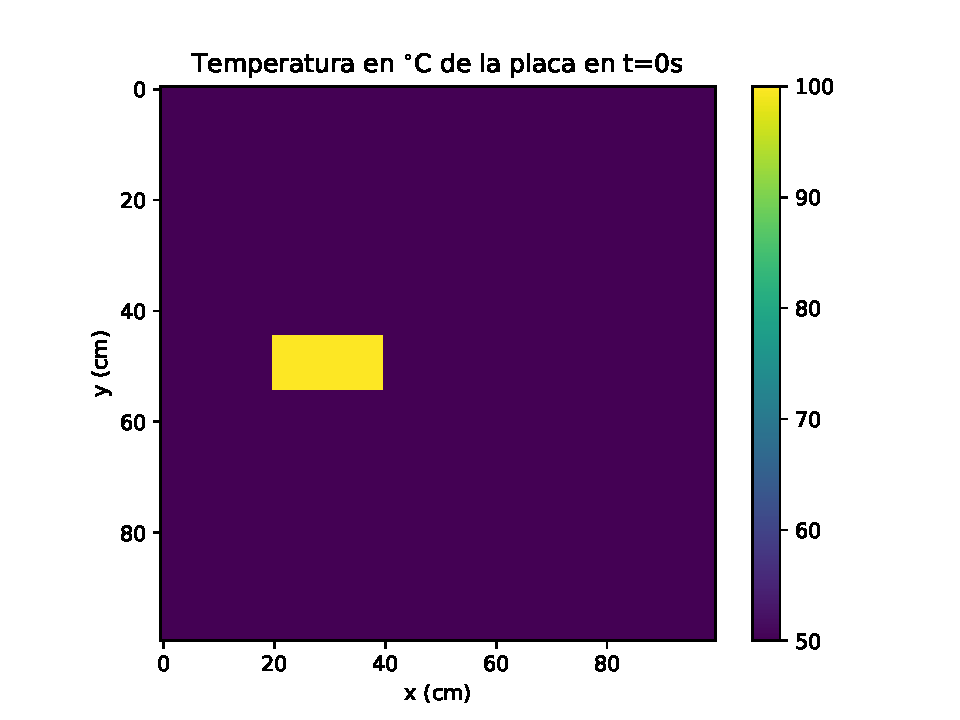
\includegraphics{p1_0.pdf}
\centering
\end{figure}

\begin{figure}[H]
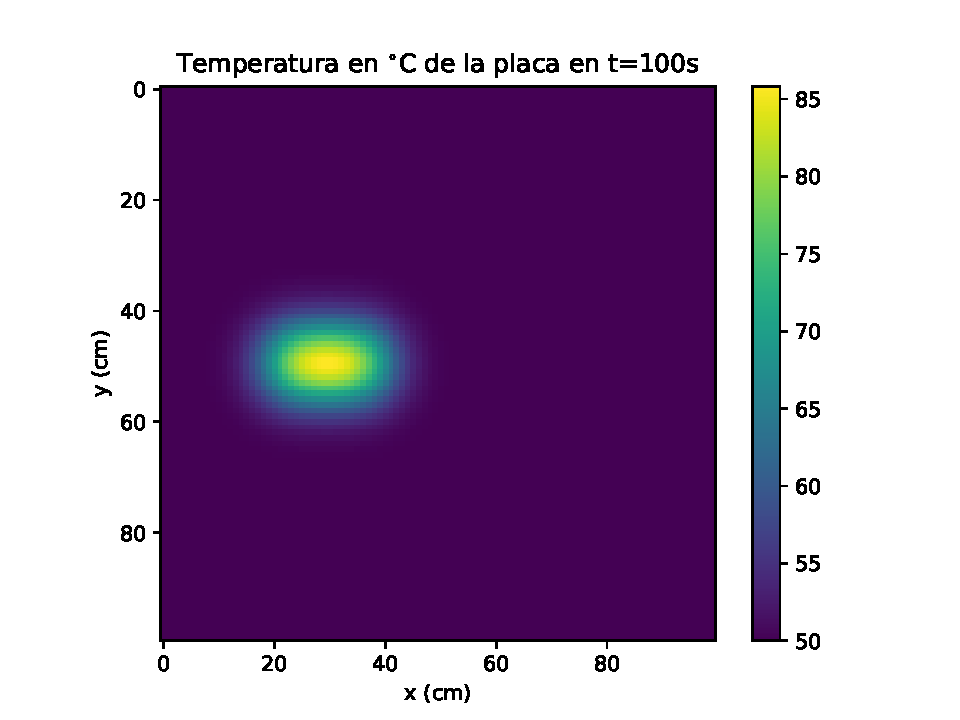
\includegraphics{p1_100.pdf}
\centering
\end{figure}

\begin{figure}[H]
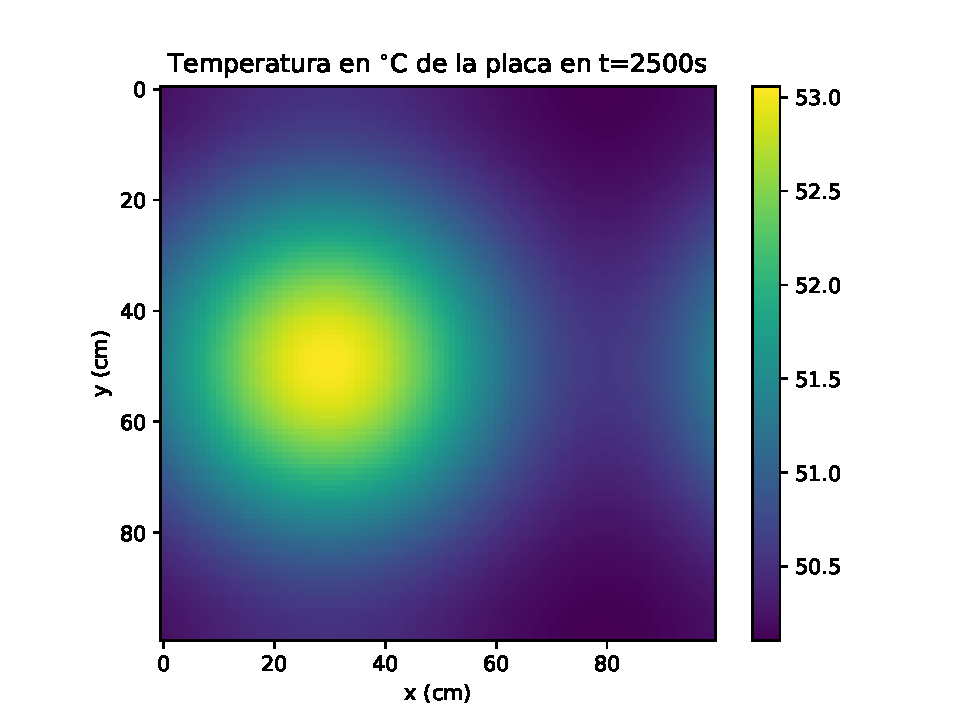
\includegraphics{p1_2500.pdf}
\centering
\end{figure}

\subsection*{Caso 2}

\begin{figure}[H]
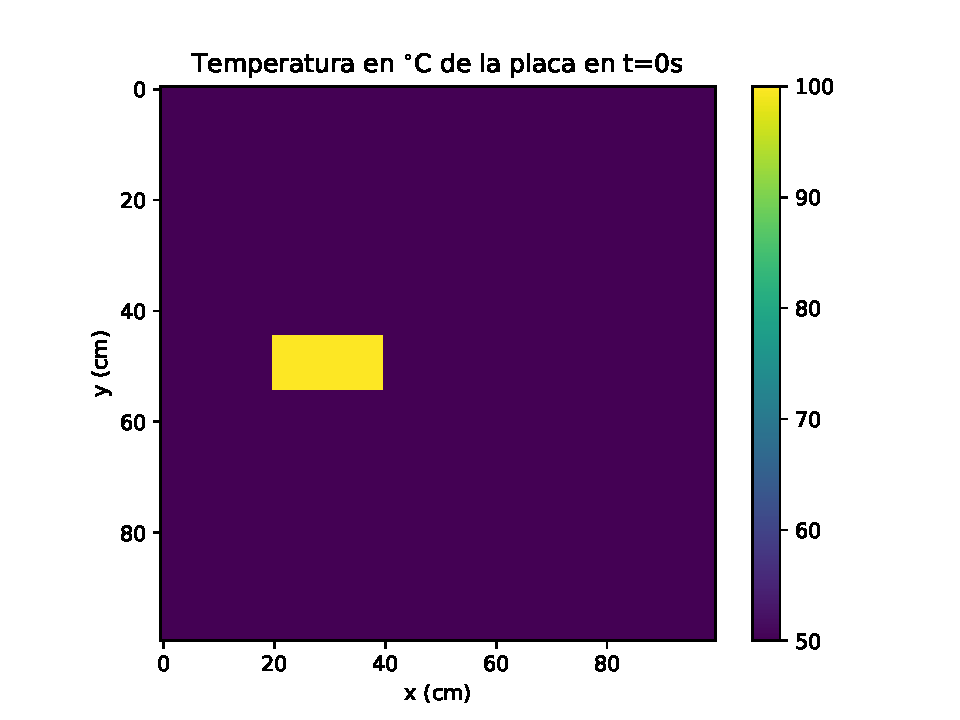
\includegraphics{p2_0.pdf}
\centering
\end{figure}

\begin{figure}[H]
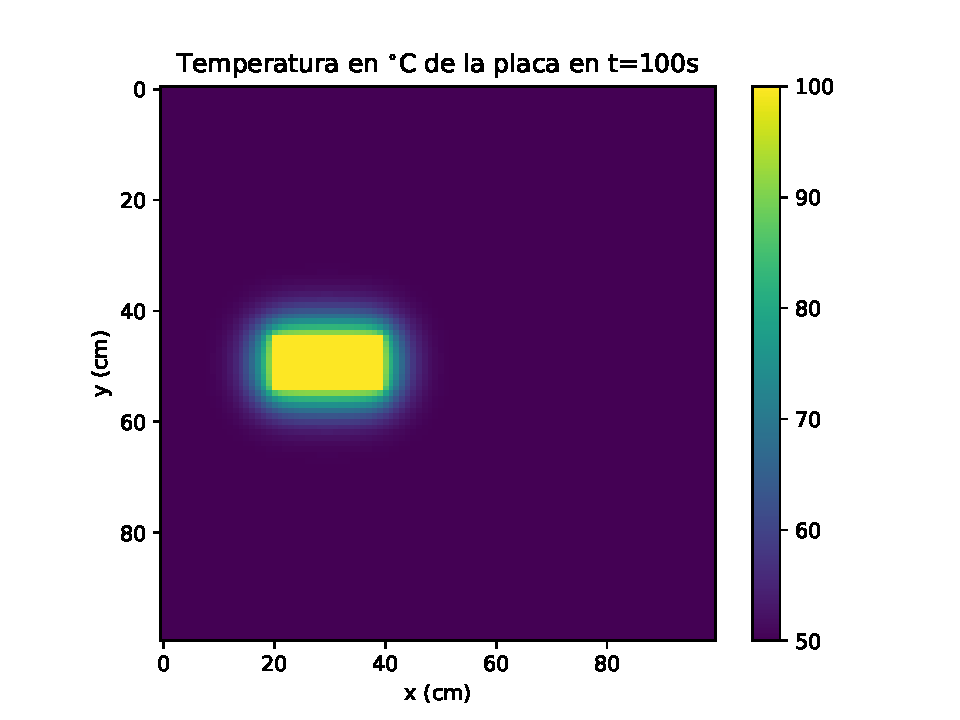
\includegraphics{p2_100.pdf}
\centering
\end{figure}

\begin{figure}[H]
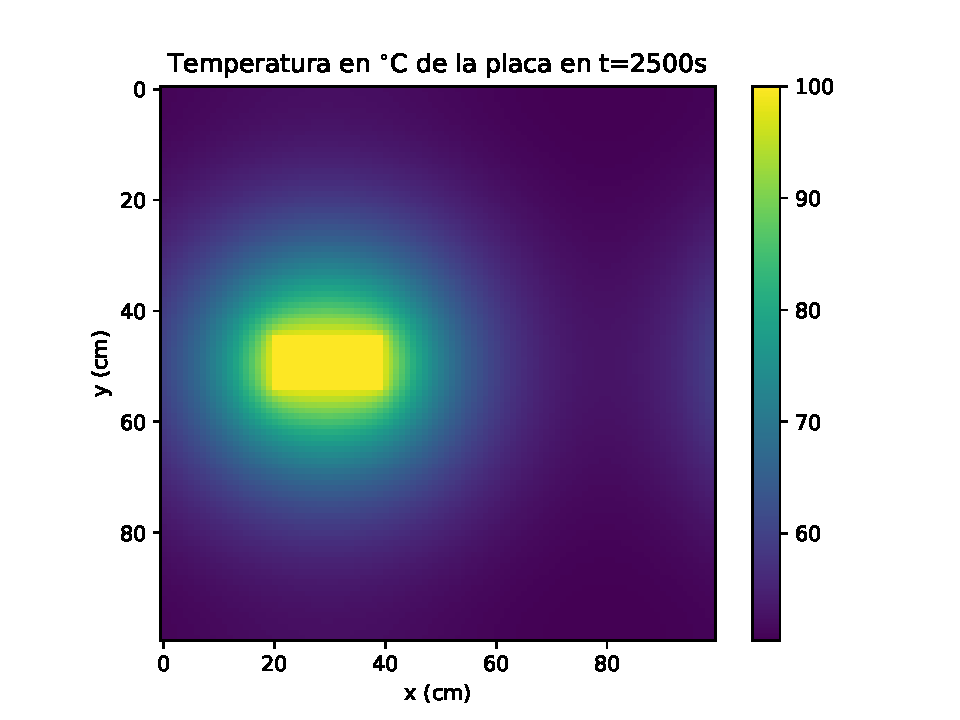
\includegraphics{p2_2500.pdf}
\centering
\end{figure}

\section*{Promedio de temperaturas}

En cada uno de los casos se calculó la temperatura promedio en función del tiempo para un total de 2500 segundos. A continuación se muestran los promedios que se obtuvieron en los casos 1 y 2 para cada una de las condiciones de frontera.\\

En las siguientes gráficas podemos notar que los cambios de temperatura promedio de las condiciones abiertas para el coeficiente de difusión tomado cambian de manera drástica respecto a cuando tomamos otro tipo de condiciones de frontera. Sin embargo, al realizar las simulaciones con distintos coeficientes $\nu$ se notaban algunos cambios, incluso en algunos casos llego a decaer, pero siempre este tipo de condiciones de frontera presentan unos promedios de temperatura mucho mayores en magnitud. Los cambios en los promedios de las otras condiciones de frontera están dentro de un rango corto y son ínfimos respecto a los cambios presentados cuando las condiciones son abiertas.

\subsection*{Caso 1}

\begin{figure}[H]
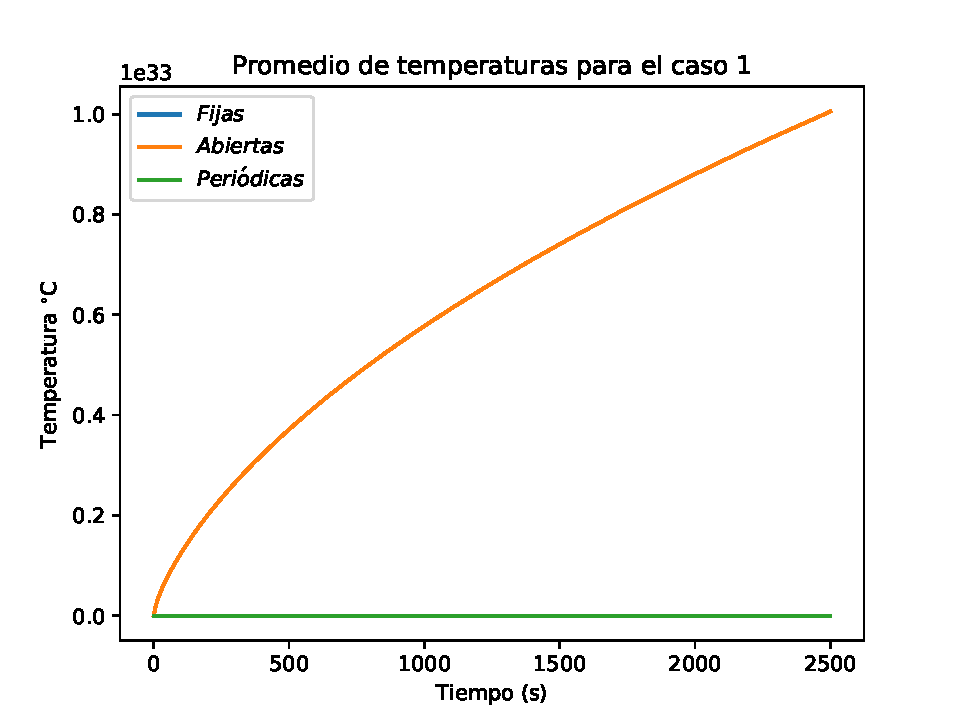
\includegraphics{prom1.pdf}
\centering
\end{figure}

\subsection*{Caso 2}

\begin{figure}[H]
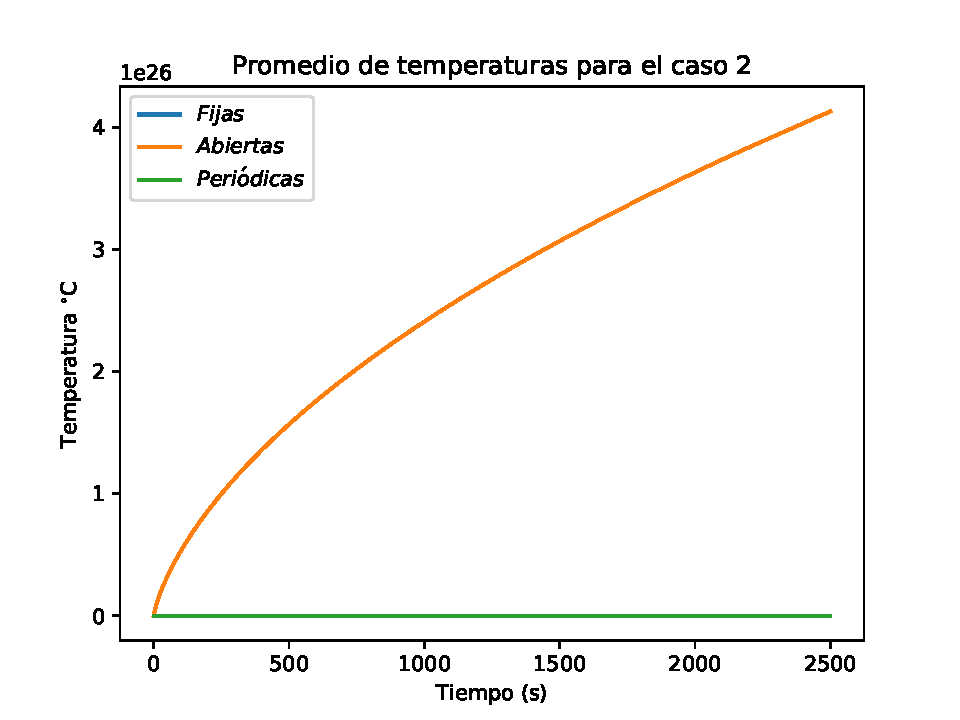
\includegraphics{prom2.pdf}
\centering
\end{figure}


\vspace{0.3cm}


\end{document}
